\documentclass{utap}

\usepackage{amsmath}
\usepackage{wrapfig}
\usepackage{xepersian}
\usepackage{lipsum}

\graphicspath{{./img/}}

\title{تمرین شماره‌ی ۵}
\author{
	\href{mailto:seyedahmadpourihosseini@gmail.com?subject=[AP\%20S98\%20A5]\%20}{احمد پوری‌حسینی},
	\href{mailto:farzadhabibii98@gmail.com?subject=[AP\%20S98\%20A5]\%20}{فرزاد حبیبی},
	\href{mailto:ahhabibvand@gmail.com?subject=[AP\%20S98\%20A5]\%20}{امیرحسین حبیب‌وند},
	\href{mailto:bardia.eghbali@gmail.com??subject=[AP\%20S98\%20A5]\%20}{بردیا اقبالی}
}
\course{برنامه‌سازی پیشرفته}
\lecturer{رامتین خسروی}
\deadline{جمعه ۶ اردیبهشت ۱۳۹۸، ساعت ۲۳:۵۵}

\begin{document}
	\maketitle

	\section{پیش‌تمرین \lr{RSDL}}

\lr{SDL} \LTRfootnote{Simple DirectMedia Layer} یک کتاب‌خانه‌ی چندسکویی، رایگان و متن‌باز است که برای بازی‌سازی و تولید برنامه‌های گرافیکی استفاده می‌شود.

کتاب‌خانه‌ی \lr{RSDL}\LTRfootnote{Ramtin SDL} یک کتاب‌خانه‌ی کمکی بسته‌بندی‌کننده\LTRfootnote{wrapper} است که امکان استفاده‌ی آسان‌تر از \lr{SDL2} را فراهم می‌کند.
نسخه‌ی فعلی \lr{RSDL} را می‌توانید از آدرس \url{https://github.com/UTAP/RSDL} دریافت کنید. همچنین، راهنمای این کتابخانه در آدرس \url{https://github.com/UTAP/RSDL/wiki} در دسترس است.

در این پیش‌تمرین برنامه‌ای ساده را با کتاب‌خانه‌ی \lr{RSDL} پیاده‌سازی می‌کنید تا بیشتر با آن آشنا شوید.  توجه کنید که این پیش‌تمرین صرفا به منظور آشنایی شما با کتاب‌خانه‌ی \lr{RSDL} بوده و تاثیری بر نمره‌‌دهی تمرین شما ندارد.


با کمک دستور \lr{\lstinline{draw_img}} و استفاده از آرگومان \lr{\lstinline{src}} آن، می توانید تکه ای از یک تصویر را روی صفحه رسم کنید. در پوشه‌ی \lr{\texttt{warmup}} تصویری از یک جدول 3×3 است که با اعداد 1 تا 9 پر شده. با استفاده از روش بالا برنامه ای بنویسید که به صورت تصادفی این جدول را به هم ریخته و روی صفحه رسم کند.

حالا می خواهیم با زدن دکمه‌ی \lr{\texttt{R}} ترتیب خانه‌ها تغییر کند. برای این کار داخل یک حلقه با استفاده از تابع \lr{\lstinline{poll_for_event}} و \lr{\lstinline{get_pressed_key}} چک کنید که آیا دکمه‌ی \lr{\texttt{R}} زده شده است یا نه. سپس مستطیل‌ها را دوباره محاسبه کنید و صفحه را به‌روزرسانی کنید.

تصویر زیر پنجره‌ی این برنامه را نشان می‌دهد.
	\begin{figure}[H]
	\begin{center}
		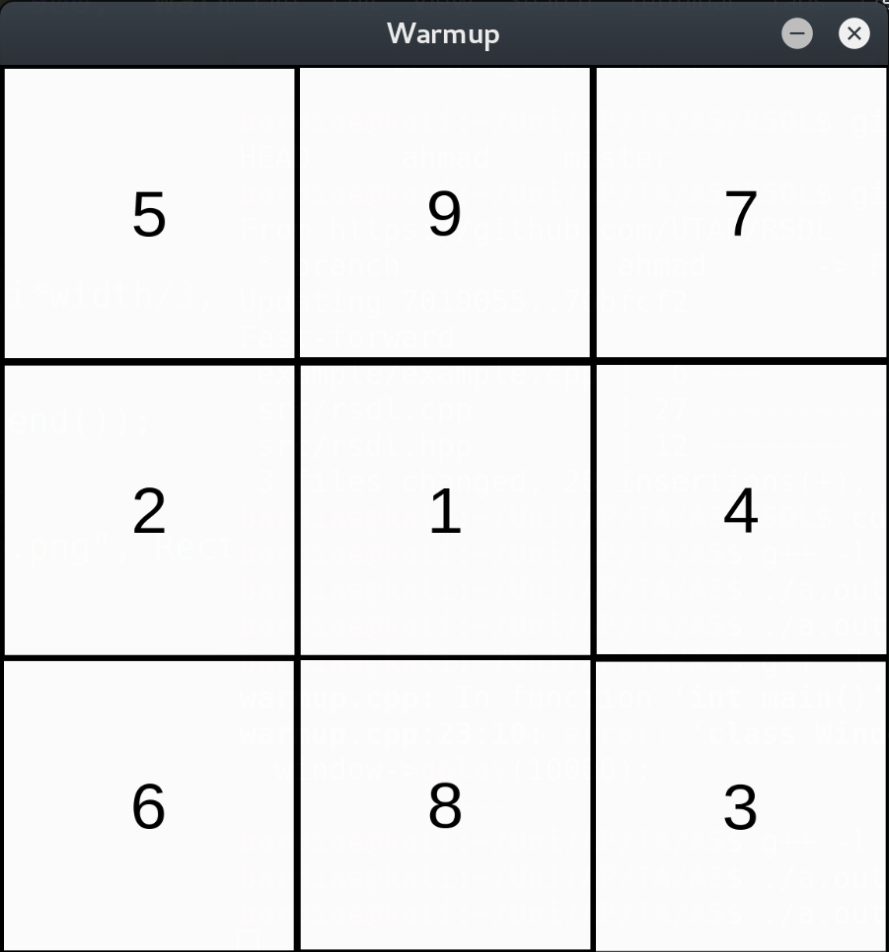
\includegraphics[width=8cm]{warmup.png}
	\end{center}
	\end{figure}
توجه کنید که این بخش برای آشنایی بیشتر شما با \lr{RSDL} است و نیازی به تحویل آن \textbf{نیست}.

	\section{سوپر ماریو}
	
	\begin{figure}[H]
		\begin{center}
			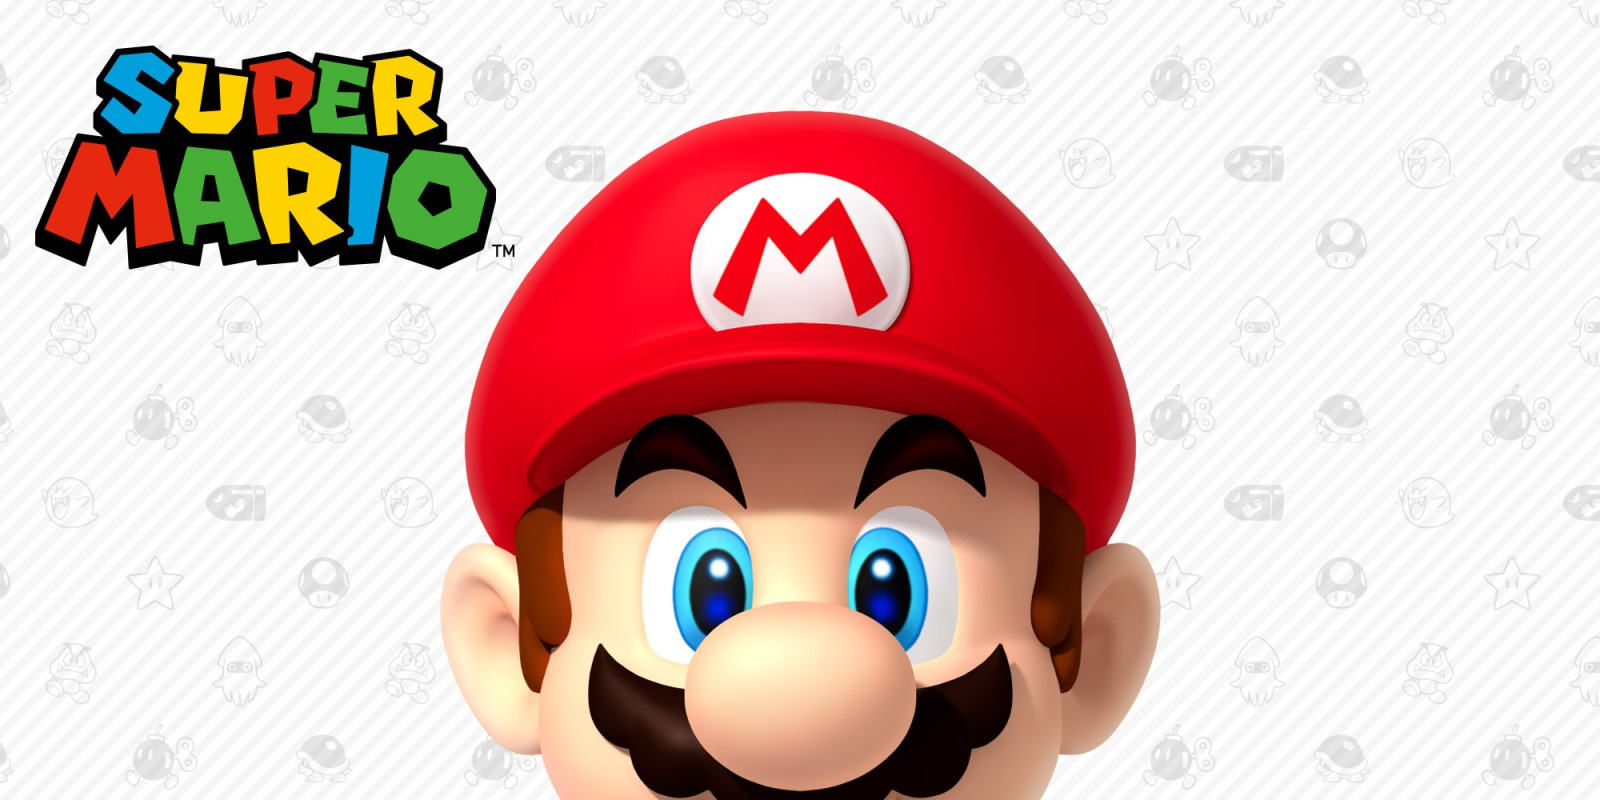
\includegraphics[width=\textwidth]{cover.jpg}
		\end{center}
	\end{figure}
سوپر ماریو نام یک سری از بازی‌های ژانر پلتفرمر \LTRfootnote{platformer} است که توسط شرکت Nintendo ساخته شده، و شامل کاراکتر بسیار مشهور ماریو است که امروزه تبدیل به نماد این شرکت شده است. این بازی به نام های \lr{Super Mario Bros} و گاهی \lr{Mario} نیز شناخته می‌شود.

بازی سوپر ماریو تشکیل شده از ماجراجویی‌های ماریو است که در دنیای خیالی امپراطوری قارچ‌ها \LTRfootnote{Mushroom Kingdom} رخ می‌دهد. مانند سایر بازی‌های ژانر پلتفرمر، بازیکن در این بازی بر روی سکو‌ها و موانعی راه می‌رود و می‌پرد که در قالب چندین مرحله‌ سامان‌دهی شده‌اند. بازی‌های این سری داستان ساده‌ای دارند که این داستان معمولا نجات شاهدخت \lr{Peach} است که توسط دشمن اصلی بازی، \lr{Bowser}، ربوده شده است.

برای تجربه کردن این بازی می‌توانید به آدرس \url{https://supermariobros.io/} مراجعه کنید که شامل یک پیاده‌سازی کامل تحت مرورگر از این بازی می‌باشد. پیشنهاد می‌کنیم که از آن استفاده کنید تا با بازی بیشتر آشنا شوید.

در این تمرین از شما انتظار می‌رود یک نسخه‌ی ساده از بازی سوپر ماریو را با توجه به توضیحاتی که در ادامه می‌آید پیاده‌سازی کنید. تمرین از چند بخش مختلف تشکیل شده است که در ادامه به توضیح هر یک می‌پردازیم.

	\subsection{نقشه}
نقشه‌ی بازی به صورت یک جدول دوبعدی از کاراکترها به شما داده می‌شود. هر کاراکتر نشان‌دهنده‌ی محتوای یک خانه \LTRfootnote{tile} از نقشه‌ی بازی است. هر خانه از نقشه‌ی معادل یک مربع در  بازی می‌باشد که تنظیم اندازه‌ی آن به عهده‌ی خودتان است، و کافی است که ظاهر بازی مشابه لینک داده شده باشد. جدول زیر معنی هر کاراکتر موجود در نقشه‌ی بازی را مشخص می‌کند.
\bgroup
    \def\arraystretch{1.5}
	\begin{table}[H]
		\centering
		\begin{center}
		\begin{tabular}{||ccc||}
            \hline
            \large\textbf{عنوان} & \large\textbf{کاراکتر معادل} & \large\textbf{تصویر}\\
             \hline
             \hline
            فضای خالی &
            \lr{\texttt{.}} &
            \\ 
            \hline

            آجر‌ساده &
             \lr{\texttt{b}} &
             \raisebox{-0.24cm}{
\includegraphics[width=0.5cm]{brick}}  \\ 
           
             \hline
            آجر شگفت‌انگیز دارای سکه &
             \lr{\texttt{?}} &
              \raisebox{-0.24cm}{
\includegraphics[width=0.5cm]{question}} 
              
              \\
              
            \hline
            آجر شگفت‌انگیز دارای قارچ قرمز یا گل آتش & \lr{\texttt{m}} &
              \raisebox{-0.24cm}{
\includegraphics[width=0.5cm]{question}} \\
            \hline
            آجر شگفت‌انگیز دارای قارچ سلامتی & \lr{\texttt{h}} & 
             \raisebox{-0.24cm}{
\includegraphics[width=0.5cm]{question}}  \\
            \hline
            بلوک معمولی & \lr{\texttt{@}} & 
             \raisebox{-0.24cm}{
\includegraphics[width=0.5cm]{block}}  \\
            \hline
            بلوک زمینی & \lr{\texttt{\#}} 
            &  \raisebox{-0.24cm}{
\includegraphics[width=0.5cm]{ground_block}}  \\
            \hline
            ماریو & \lr{\texttt{M}} & 
            \raisebox{-0.24cm}{
\includegraphics[width=0.5cm]{mario}}\\
            \hline
            گومبا کوچولو & \lr{\texttt{l}} &
             \raisebox{-0.24cm}{
\includegraphics[width=0.5cm]{goomba}} \\
            \hline
            کوپا~تروپا & \lr{\texttt{k}} &
             \raisebox{-0.27cm}{
\includegraphics[width=0.5cm]{koopa}} \\
            \hline
            لوله  & \lr{\texttt{|}} &
             \raisebox{-0.14cm}{
\includegraphics[width=0.3cm]{pipe1}}
             \raisebox{-0.14cm}{
\includegraphics[width=0.3cm]{pipe2}} 
             \raisebox{-0.14cm}{
\includegraphics[width=0.3cm]{pipe3}}
             \raisebox{-0.14cm}{
\includegraphics[width=0.3cm]{pipe4}}   \\
            \hline
            پرچم & \lr{\texttt{f}} & 
            \raisebox{-0.24cm}{
\includegraphics[width=0.5cm]{flag1}}
            \raisebox{-0.24cm}{
\includegraphics[width=0.5cm]{flag2}}  \\
            \hline
		\end{tabular}
		\end{center}
	\end{table}
\egroup
عکس‌های مربوط را می‌توانید در پوشه‌ی \lr{\texttt{assets}} پیدا کنید. همچنین عکس پس‌زمینه‌ نیز داخل همین پوشه قرار دارد که باید پشت تمامی تصاویر دیگر رسم شود.

توجه کنید که پیاده‌سازی شما نباید به یک نقشه‌ی خاص برای بازی وابسته باشد و باید بتواند با هر نقشه‌ی دلخواهی که مطابق فرمت گفته شده باشد، \textbf{بدون نیاز} به ترجمه‌ی\LTRfootnote{compile} مجدد، اجرا شود. به این  منظور برنامه‌ی شما باید آدرس نقشه‌ی مرحله‌ی مورد نظر را از خط‌فرمان\LTRfootnote{command line} دریافت کند. در هنگام تحویل تمرین، برنامه‌ی شما با یک نقشه‌ی جدید که قبلاً ندیده‌اید آزموده خواهد شد.

	\subsection{دوربین}
نقشه‌ی بازی از ناحیه‌ای که دوربین بازی می‌تواند نشان دهد، بسیار بزرگ‌تر است. در نتیجه نیاز است که با حرکت ماریو به سمت جلو، دوربین نیز او را دنبال بکند. یعنی وقتی ماریو به لبه‌ی راستی صفحه نزدیک می‌شود باید دوربین نیز کمی به راست برود تا ماریو از صفحه خارج نشود. اینکه مرز این جابه‌جایی دوربین چقدر باشد به عهده‌ی خود شما است و صرفاً طبیعی بودن آن کافی است.

توجه کنید که ماریو هیچ گاه نباید بتواند از لبه‌ی سمت چپ صفحه خارج شود، در نتیجه دوربین هیچ‌گاه نیاز نیست به سمت چپ حرکت کند.

نگران خارج شدن ماریو در راستای عمودی صفحه نیز نباشید، نقشه‌هایی که در اختیار شما قرار می‌گیرند نیازی به جابه‌جایی دوربین در این راستا نخواهند داشت.

همچنین در نظر داشته باشید که عکس پس‌زمینه بازی هم باید حرکت کند. در واقع در هر لحظه باید بخشی از آن را نمایش دهید و با جابه‌جایی دوربین بخش بعدی عکس را به کاربر نمایش دهید تا حس حرکت در کاربر القا شود.
	\subsection{حرکات}
		\subsubsection{ماریو}
			\begin{figure}[H]
			\begin{center}
				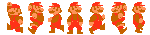
\includegraphics[width=0.7\textwidth]{marioWalk}
			\end{center}
		\end{figure}
حرکات ماریو در این بازی بسیار ساده هستند. ماریو باید با فشار دادن کلید‌های \lr{\texttt{d}} و \lr{\texttt{a}} به ترتیب به سمت راست و چپ حرکت کند، وهم‌چنین با فشار دادن کلید \lr{\texttt{w}} بپرد. توجه کنید که ساختار جدول‌مانند نقشه، فقط به منظور راحتی ذخیره کردن و خواندن نقشه است و حرکت‌های داخل بازی ریزدانه‌تر از خانه‌های نقشه و در مقیاس پیکسل هستند. حرکت ماریو در راستای محور \lr{y}‌ها همواره از فرمول‌های حرکت با شتاب ثابت پیروی می‌کند، یعنی:
	\begin{gather*}
		\Delta y = v_y \Delta t\\
		\Delta v_y = g \Delta t
	\end{gather*}
و حرکت در راستای محور \lr{x}‌ها نیز از فرمول حرکت با سرعت ثابت تبعیت می‌کند، یعنی:
	\begin{gather*}
		\Delta x = v_x \Delta t
	\end{gather*}
که در این فرمول‌ها $v_y$ و $v_x$ به ترتیب سرعت در راستای \lr{y} و سرعت در راستای \lr{x} بوده و $g$ شتاب گرانشی است.

معمولاً فرمول‌های سقوط آزاد را به شکل
$y = -\frac{1}{2}gt^2 + v_{0_y} t + y_0$
می‌بینیم، که برای محاسبه‌ی مستقیم جابه‌جایی آسان‌تر است ولی استفاده از فرمول‌های بالا برای پیاده‌سازی کامپیوتری راحت‌تر هستند.

در واقع فشار دادن دکمه‌ی پرش باعث ایجاد یک سرعت اولیه در راستای‌ \lr{y} می‌شود که طی زمان با توجه به ثابت $g$ از آن کاسته می‌شود. مشخص کردن مقدار دقیق ثابت $g$ و مقدار $v_x$ به عهده‌ی خود شما است و لازم و کافی است که این مقادیر طوری انتخاب شوند که حرکت ماریو طبیعی بوده و مشابه لینک داده شده در ابتدای تمرین باشد. طبیعتاً این فرمول‌ها فقط در حالتی برقرار هستند که مانعی در سر راه ماریو وجود نداشته باشد، چرا که در این صورت حرکت ماریو در آن راستا متوقف می‌شود.
		\subsubsection{دشمنان}
در این بازی از شما خواسته می‌شود که دو نوع دشمن را پیاده‌سازی کنید. توضیحات این دو نوع در بخش دشمنان آمده است. اما همه‌ی دشمنان ویژگی‌های مشترکی در حرکت خود دارند که در این بخش به آن‌ها می‌پردازیم.

دشمنان در این بازی در ابتدا در مکان اولیه‌ی خود ساکن هستند و در همین وضعیت می‌مانند تا وقتی که وارد کادر دوربین بازی شوند. پس از ورود به کادر دوربین دشمنان شروع به حرکت به سمت چپ کرده و تا وقتی مانعی جلو‌ی آن‌ها نباشد به حرکت خود ادامه می‌دهند. هر وقت که دشمنی به مانعی در مسیر حرکت خود برخورد کند، جهت حرکت خود را تغییر می‌دهد.

برخلاف بازی اصلی، در این تمرین دشمنان برای هم مانع نیستند، یعنی دشمنان می‌توانند از یکدیگر عبور کنند. تنظیم سرعت حرکت دشمنان نیز، مانند ماریو، بر عهده‌ی خود شما است و کافی است که حرکت و سرعت دشمنان طبیعی و مشابه لینک داده شده در ابتدای تمرین باشد.

از شما انتظار می‌رود با استفاده از عکس‌های داده شده، حس اینکه ماریو و دشمنان در حرکت پاهای خود را تکان می‌دهند را به‌وجود بیاورید.

	\subsection{موانع}
در این بازی سه مانع مختلف وجود دارد، که جلوی ورود ماریو را به خانه‌ای که داخل آن هستند می‌گیرند:

	\begin{itemize}
		\begin{minipage}{.75\textwidth}
		\item
\textbf{بلوک‌ها}
ساده‌ترین موانع موجود در بازی. اندازه‌ی آن‌ها همیشه به اندازه‌ی یک خانه‌ از نقشه‌ی بازی است. بلوک‌ها خود دو نوع معمولی و زمینی دارند، که تفاوت آن‌ها فقط در ظاهرشان است. این تفاوت را می‌توانید در جدول بخش نقشه‌ی بازی مشاهده کنید.
\end{minipage}
\begin{minipage}{.15\textwidth}
\begin{figure}[H]
	\begin{center}
		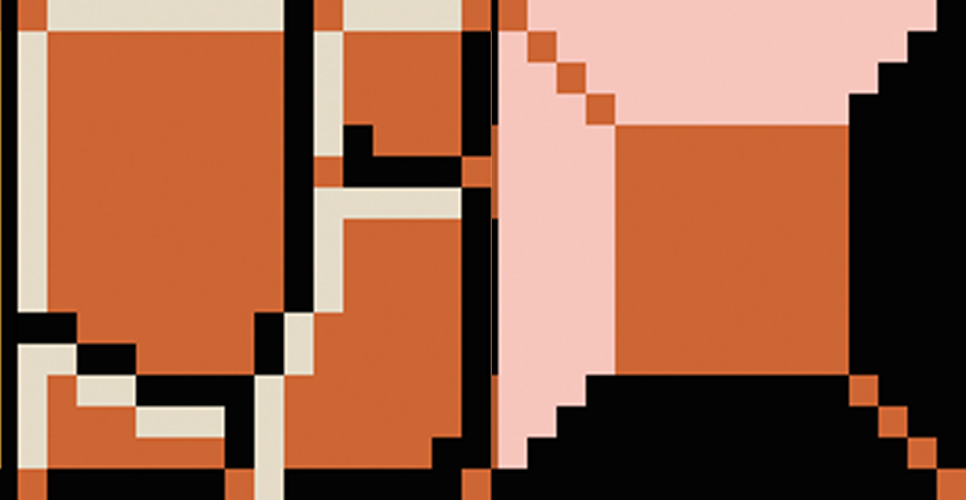
\includegraphics[width=1.8cm]{blocks}
	\end{center}
\end{figure}
\end{minipage}

\begin{minipage}{.75\textwidth}
		\item
		
\textbf{لوله‌ها}
این موانع کمی از بلوک‌ها پیچیده‌تر هستند. ارتفاع این موانع می‌تواند تا حد دلخواه زیاد باشد، ولی عرض آن‌ها همواره برابر دو خانه‌ از نقشه است. همچنین این موانع همواره عمودی هستند. شما باید از عکس‌های داده شده استفاده کنید، تا ظاهر لوله را مشابه لینک داده شده در ابتدای تمرین بسازید.
\end{minipage}
\begin{minipage}{.15\textwidth}
\begin{figure}[H]
	\begin{center}
		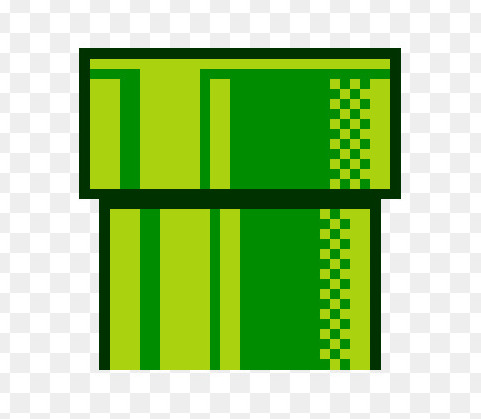
\includegraphics[width=1.8cm]{allPipes}
	\end{center}
\end{figure}
\end{minipage}
		\item
\textbf{آجرها}
این موانع، بر خلاف دو مانع قبلی که روی زمین هستند، همواره از زمین فاصله دارند. وقتی ماریو از پایین به آجری ضربه می‌زند، آجر کمی به بالا پرتاب می‌شود و اگر دشمنی روی آن‌ باشد، آن را از بین می‌برد، سپس به موقعیت اول خود برمی‌گردد. آجرها ۲ نوع مختلف به شرح زیر دارند:
		\begin{itemize}
					\begin{minipage}{.75\textwidth}
			\item
\textbf{معمولی}
این آجرها از آجر‌های شگفت‌انگیز ضعیف‌ترند. به این معنا که به هنگام ضربه زدن ماریو به آن‌ها از پایین، اگر ماریو بزرگ باشد، می‌شکنند. این آجر‌ها هیچ‌وقت محتوایی ندارند.
\end{minipage}
\begin{minipage}{.1\textwidth}
\begin{figure}[H]
	\begin{center}
		
\includegraphics[width=0.9cm]{brick}
	\end{center}
\end{figure}
\end{minipage}

\begin{minipage}{.7\textwidth}
			\item
\textbf{شگفت‌انگیز}
این آجرها که با علامت سؤال مشخص شده‌اند، محکم هستند و هیچ‌گاه نمی‌شکنند. اما وقتی ماریو از پایین به آن‌ها ضربه میزند، محتوای آن‌ها بیرون می‌آید. پس از بیرون آمدن محتوایشان،‌ این آجر‌ها تغییر شکل داده و علامت سؤالشان از بین می‌رود.

\end{minipage}
\begin{minipage}{.15\textwidth}
\begin{figure}[H]
	\begin{center}
		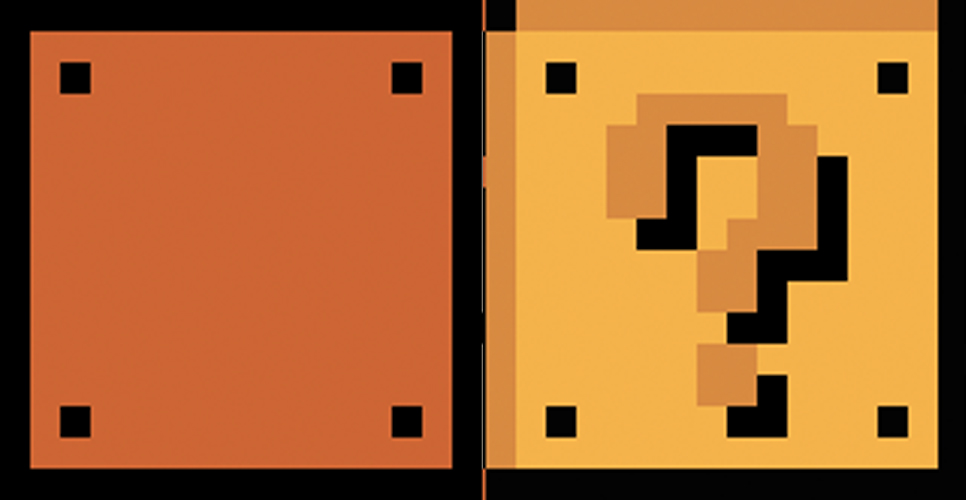
\includegraphics[width=1.8cm]{magicBricks}
	\end{center}
\end{figure}
\end{minipage}

		\end{itemize}
	\end{itemize}


	\subsection{دشمنان}
در این بازی دو نوع دشمن وجود دارد، که قبل از اینکه به ویژگی‌های هر یک بپردازیم، ابتدا ویژگی‌های مشترک دشمنان را بررسی می‌کنیم.
همه‌ی دشمنان، همانطور که در بخش حرکت توضیح داده شد، وقتی که وارد کادر بازی می‌شوند، به طور خودکار شروع به حرکت به سمت چپ می‌کنند.
وقتی ماریو به یکی از دشمنان برخورد کند، اگر این برخورد از بالای سر دشمن باشد، آن دشمن آسیب می‌بیند، ولی ماریو آسیبی نمی‌بیند و در عوض فقط کمی به بالا پرتاب می‌شود. این پرتاب رو به بالا مانند پرشی با قدرت کم است. اما اگر این برخورد از جهتی دیگر باشد، ماریو یک جان خود را از دست داده و به ابتدای مرحله برمی‌گردد. دشمنان این بازی عبارتند از:
	\begin{itemize}
	
		\begin{minipage}{.75\textwidth}
		\item

\textbf{گومبا کوچولو (\lr{Little Gomba})}
گومباها ساده‌ترین دشمنان در این بازی هستند. این دشمنان به محض برخورد با ماریو از بالای سرشان از بین می‌روند. البته قبل از اینکه کامل از بازی حذف شوند، برای چند ثانیه بدن مرده‌ی آن‌ها روی زمین باقی می‌ماند و پس از مدت کوتاهی دیگر اثری از آن‌ها در بازی باقی نمی‌ماند.
\end{minipage}
\begin{minipage}{.15\textwidth}
\begin{figure}[H]
	\begin{center}
		
\includegraphics[width=0.9cm]{goomba}
	\end{center}
\end{figure}
\end{minipage}


		\begin{minipage}{.75\textwidth}
		\item
\textbf{کوپا~تروپا (\lr{Koopa Troopa})}
این دشمنان کمی پیچیده‌ترند. وقتی ماریو از بالا به کوپا~تروپا برخورد می‌کند کوپا~تروپا به صورت برعکس روی زمین قرار می‌گیرد و دیگر حرکت نخواهد کرد. با برخورد بعدی ماریو با کوپا~تروپا از سمت بالا، این موجود در جهت مناسب پرتاب می‌شود. در این حالت، کوپا~تروپا با هر چیزی که برخورد کند، آن را بلافاصله می‌کشد (کوپا~تروپاهای دیگر نیز بلافاصله می‌میرند و برعکس روی زمین نمی‌افتند) و مشابه تمامی حرکت‌های دیگر، وقتی تروپا در این حالت به مانعی برخورد بکند، جهت حرکتش عوض می‌شود. و این حالت تا جایی ادامه دارد که کوپا~تروپا از یک جای خالی در نقشه بیرون بیفتد و از نقشه خارج شود.
\end{minipage}
\begin{minipage}{.15\textwidth}
\begin{figure}[H]
	\begin{center}
		
\includegraphics[width=0.9cm]{koopa}
	\end{center}
\end{figure}
\end{minipage}

	\end{itemize}

	\subsection{محتوای آجرها}
همانطور که در بخش موانع گفته شد، آجر‌های شگفت‌انگیز می‌توانند محتویاتی داشته باشند، که به هنگام ضربه زدن ماریو به آن‌ها از سمت پایین، این محتوا از آن‌ها خارج می‌شود. این محتوا می‌تواند یکی از موارد زیر باشد:
	\begin{itemize}
			\begin{minipage}{.75\textwidth}
		\item
				
\textbf{سکه}
وقتی ماریو به آجر دارای سکه ضربه می‌زند، باید یک نشانه‌ی بصری برای اینکه سکه‌ای داخل آن آجر وجود داشت (مثلا اینکه یک سکه از آجر خارج شود) ظاهر شود و سپس یکی به تعداد سکه‌های ماریو اضافه شود.
\end{minipage}
\begin{minipage}{.15\textwidth}
\begin{figure}[H]
	\begin{center}
		
\includegraphics[width=0.9cm]{coin}
	\end{center}
\end{figure}
\end{minipage}

	\begin{minipage}{.75\textwidth}
		\item
\textbf{قارچ قرمز}
این قارچ‌ها همانطور که از اسمشان پیداست، قارچ‌های قرمزی هستند که ماریو با خوردن آن‌ها بزرگ‌تر می‌شود.
\end{minipage}
\begin{minipage}{.15\textwidth}
	\begin{figure}[H]
		\begin{center}
			
\includegraphics[width=0.9cm]{red}
		\end{center}
	\end{figure}
\end{minipage}

این تغییر اندازه باعث می‌شود که ماریو بتواند:
		\begin{itemize}
			\item
توانایی شکستن آجر‌ها را داشته باشد.
			\item
در برابر یک ضربه از دشمنان ایمن باشد و در صورت اصابت هرگونه ضربه تنها اندازه‌اش کوچک‌تر شود و از جان‌های او کم نشود. توجه کنید که بلافاصله پس از این برخورد، ماریو باید حدود یک ثانیه غیرقابل‌کشتن باشد. در طول این مدت ماریو و دشمنان هیچ تاثیری نمی‌توانند بر‌یکدیگر بگذارند.
		\end{itemize}
		این قارچ‌ها وقتی به وجود می‌آیند که ماریو به یک آجر دارای قارچ قرمز یا گل آتش ضربه بزند، در حالی که اندازه‌ی آن در حالت عادی است.

	\begin{minipage}{.75\textwidth}
		\item
\textbf{قارچ جان}
ماریو با خوردن این قارچ یک جان به جان‌هایش اضافه می‌شود.
\end{minipage}
\begin{minipage}{.15\textwidth}
\begin{figure}[H]
	\begin{center}
		
\includegraphics[width=0.9cm]{health}
	\end{center}
\end{figure}
\end{minipage}

توجه کنید که قارچ‌ها پس از خروج از آجر، مانند دشمنان به طور اتوماتیک شروع به حرکت می‌کنند. البته جهت حرکت آن‌ها در ابتدا رو به راست است. همانند دشمنان، قارچ‌ها نیز در صورت برخورد با مانع افقی، جهت حرکت خود را تغییر می‌دهند.
	
	\begin{minipage}{.75\textwidth}
		\item
		\textbf{گل آتش} \textit{(امتیازی)}
		وقتی که ماریو به یک آجر دارای قارچ قرمز یا گل آتش ضربه بزند، در حالی که اندازه‌ی ماریو بزرگ است، به جای قارچ قرمز، یک گل آتش از آجر خارج می‌شود. ماریو با خوردن این گل، سفید رنگ می‌شود، و می‌تواند با فشردن دکمه‌ی x گلوله‌ای آتشین به سمت روبه‌روی خود پرتاب کند که در صورت برخورد با دشمنان آن‌ها را می‌کشد. اگر ماریو در این حالت با دشمنی برخورد کند، به رنگ و اندازه‌ی عادی خود برمی‌گردد.
	\end{minipage}
	\begin{minipage}{.15\textwidth}
		\begin{figure}[H]
			\begin{center}
				
\includegraphics[width=0.9cm]{flower}
			\end{center}
		\end{figure}
	\end{minipage}
	

	\end{itemize}

	\subsection{سربرگ‌ بازی}

در طول بازی، باید اطلاعات مشخصی در بالای صفحه در قالب یک سربرگ\LTRfootnote{header} نمایش داده شوند. این اطلاعات به شرح زیرند:
	\begin{itemize}
		\item
\textbf{سکه‌ها}\LTRfootnote{coins}
تعداد سکه‌هایی که تا به آن لحظه توسط ماریو جمع‌آوری شده است.
		\item
\textbf{جان‌ها}\LTRfootnote{lives}
تعداد جان‌های باقی‌مانده‌ی ماریو. در ابتدا تعداد جان‌های ماریو  ۳ است.
	\begin{figure}[H]
	\begin{center}
		
\includegraphics[width=0.8\textwidth]{header}
	\end{center}
\end{figure}

	\end{itemize}

	\subsection{پایان بازی}
هر بار که ماریو با یکی از دشمنان برخورد می‌کند یا از پایین صفحه به بیرون سقوط می‌کند،  اگر از جان‌های ماریو باقی مانده باشد، باید ماریو به ابتدای مرحله بازگشته و یکی از جان‌های او کم شود. به جز این دو مورد (جان و مکان ماریو)، تغییر دیگری نباید در وضعیت مرحله (از جمله خالی یا پر بودن آجر‌ها، اینکه کدام دشمن‌ها مرده اند و غیره) داده شود.

اگر برای ماریو جانی باقی نمانده باشد، باید با نشان دادن پیغام \lr{You Lose} بازی تمام شود.

اگر ماریو بتواند به پرچم انتهای مرحله برسد، بازیکن بازی را برده است یا نمایش پیغام \lr{You Win} بازی خاتمه می‌یابد.
	\subsection{نکات پایانی}
	\begin{itemize}
		\item
در بازی اصلی، اصطکاک ماریو با زمین به حدی نیست که وقتی کاربر دستش را از روی دکمه‌ی راست/چپ برداشت ماریو بلافاصله از حرکت بایستد. همچنین موقع شروع حرکت نیز سرعت ماریو به تدریج زیاد می‌شود تا به سقف خود برسد. در واقع ماریو در بازی اصلی روی سطح سر می‌خورد. پیاده‌سازی سُر بودن سطح زمین بازی را جذاب‌تر می‌کند و انجام آن اختیاری بوده و برای شما نمره‌ی امتیازی خواهد داشت. (در این حالت دیگر حرکت ماریو در راستای x از فرمول حرکت با سرعت ثابت تبعیت نمی‌کند.)
		\item
اینکه آجر‌های شگفت‌انگیز بین سه رنگ موجود به صورت چرخشی تغییر رنگ بدهند (مانند آنچه که در لینک نمونه هست) برای شما نمره‌ی امتیازی خواهد داشت.
	\item
	در داخل پوشه‌ی \lr{\texttt{sound}}، موسیقی پس‌زمینه‌ی بازی اصلی به همراه تعدادی \lr{sound effect} قرار گرفته است. شما می‌توانید با استفاده از امکانات پخش موسیقی \lr{RSDL} به بازی خود صدا نیز اضافه کنید. انجام این کار امتیازی است.
	\item
	در این بازی به شما چهار مورد معرفی شده که در صورت پیاده‌سازی آن‌ها به شما نمره‌ی امتیازی داده خواهد شد. این موارد و نمره‌ی امتیازی هر کدام عبارتند از:
    \begin{itemize}
\item گل آتش \dotfill ۱۰ نمره
\item سر خوردن ماریو \dotfill ۱۲ نمره
\item صدا گذاری بازی \dotfill ۱۲ نمره
\item تغییر رنگ چرخشی آجر‌های شگفت‌انگیز \dotfill ۳~ نمره
    \end{itemize}
همچنین حداکثر ۵ نمره برای جذاب‌تر و زیباتر بودن پیاده‌سازی از حداقل قابل‌قبول ممکن است به شما تعلق بگیرد.

توجه کنید که حداکثر نمره‌ی قابل دریافت از این تمرین ۱۲۵ نمره است و با پیاده‌سازی بخش‌های امتیازی مختلف نمره‌ای بیش از این مقدار دریافت نخواهید کرد.
		\item
در صورت نیاز می‌توانید ساختار تمامی پرونده‌های\LTRfootnote{file} مورد نیاز برای بازی (از جمله تصاویر و پرونده‌های نقشه) را تغییر دهید و لزومی ندارد ساختار اولیه را حفظ کنید.
توجه کنید که ممکن است کتاب‌خانه‌ی \lr{RSDL} به‌روزرسانی شود؛ پس سعی کنید تغییری در کتابخانه ایجاد نکنید.
	
	\end{itemize}

\section{نحوه‌ی تحویل}
    پرونده‌‌های مربوط به برنامه‌ی خود را در پرونده‌ای با نام \lr{A5-SID.zip} در صفحه‌ی \lr{CECM} درس بارگذاری کنید که \lr{SID} شماره‌ی دانشجویی شماست؛ برای مثال اگر شماره‌ی دانشجویی شما ۸۱۰۱۹۷۹۹۹ باشد، نام پوشه‌ی شما باید \lr{A5-810197999.zip} باشد.
    \begin{itemize}
        \item
برنامه‌ی شما باید در سیستم‌عامل لینوکس و با مترجم \lr{g++} با استاندارد \lr{\texttt{c++11}} ترجمه و اجرا شود. این مسئله را در هنگام نوشتن \lr{makefile} در نظر بگیرید.
	\item
برنامه شما باید حتما طراحی شی‌گرا داشته باشد. همچنین باید به صورت \lr{Multifile} باشد و استفاده از \lr{Makefile} در این تمرین اجباری است.
	\item
برای ایجاد رابط کاربری گرافیکی\LTRfootnote{GUI} و تمامی افکت‌های صوتی و تصویری برنامه‌ی خود باید از کتاب‌خانه‌ی \lr{SDL2} و کتاب‌خانه‌ی \lr{RSDL} استفاده کنید.
        \item
پرونده‌ای که بارگذاری می‌کنید باید نسخه‌ی فشرده‌ی پوشه‌ی کامل تمرین باشد که شامل کد کامل برنامه‌ی شما به همراه کتاب‌خانه‌ی \lr{RSDL}، تصاویر و - در صورت استفاده - پرونده‌های صوتی است.
        \item
هدف این تمرین یادگیری شماست. لطفاً تمرین را خودتان انجام دهید. در صورت کشف تقلب مطابق قوانین درس با آن برخورد خواهد شد.
    \end{itemize}
\end{document}
